% Copyright (c) 2021 Eclipse Arrowhead Project
%
% This program and the accompanying materials are made available under the
% terms of the Eclipse Public License 2.0 which is available at
% http://www.eclipse.org/legal/epl-2.0.
%
% SPDX-License-Identifier: EPL-2.0

The \GlossaryHyperRef{framework-arrowhead}{Arrowhead framework} is two things, as depicted in Figure \ref{fig:framework}.
Firstly, it is a framework of assumptions, concepts, values and practices that frame the problem domain of \textit{dynamic device coordination in the context of automation}.
Secondly, it is a set of software specifications, \GlossaryHyperRef{implementation-software}{implementations} and other \GlossaryHyperRef{artifact}{artifacts} meant to help address that problem domain.
In this section, we provide an overview of the primary \textit{concepts} of the Arrowhead framework.
While \textit{assumptions} and \textit{values} may be possible derive from this overview, neither of these, nor the other parts of the framework, are considered directly.

\vspace*{1mm}

\begin{figure}[ht!]
  \centering
  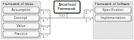
\includegraphics[scale=0.9]{figures/framework}
  \caption{
    The two main categories of concerns of the arrowhead framework: ideas and software.
  }
  \label{fig:framework}
\end{figure}

\vspace*{-3mm}

\subsection{Stakeholders and Artifacts}

There are two kinds of citizens in the world of Arrowhead, (1) \GlossaryHyperRef{stakeholder}{stakeholders} and (2) \GlossaryHyperRef{artifact}{artifacts}, as depicted in Figure \ref{fig:world}.
The former denotes a person or organization engaged in an Arrowhead enterprise, while the latter is any thing or object, tangible or intangible, that could be relevant to consider as part of such an enterprise.
Stakeholders \GlossaryHyperRef{owner}{own}, \GlossaryHyperRef{designer}{design}, \GlossaryHyperRef{developer}{develop}, \GlossaryHyperRef{operator}{operate}, and \GlossaryHyperRef{user}{use} artifacts, among many other possible activities.
It is their business needs and ambitions that dictate what and how Arrowhead artifacts will be employed.

\vspace*{1mm}

\begin{figure}[ht!]
  \centering
  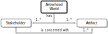
\includegraphics[scale=0.9]{figures/world}
  \caption{
    The two kinds of citizens of the Arrowhead world: stakeholders and artifacts.
  }
  \label{fig:world}
\end{figure}

\vspace*{-3mm}

\subsection{Devices, Systems and Services}

The most essential types of Arrowhead artifacts are (1) \GlossaryHyperRef{device}{devices}, (2) \GlossaryHyperRef{system}{systems} and (3) \GlossaryHyperRef{service}{services}, as shown in Figure \ref{fig:device-system-service}.
\textit{Devices} constitute the physical machines that make up the industrial complexes, vehicles, tools, and other things that could be made operational via Arrowhead.
Each device hosts one or more \textit{systems}, which are \GlossaryHyperRef{communication}{communicating} \GlossaryHyperRef{instance-software}{software instances} that make their devices work toward whatever goals are set for them.
Finally, a \textit{service} is a set of related \GlossaryHyperRef{function-service}{functions} that a system can make its device perform for a person or another system.
Services can be concerned with manufacturing, repair, analysis, or any other physical or virtual activity.
The service is the primary means whereby systems coordinate to fulfill their assignments.

\vspace*{1mm}

\begin{figure}[ht!]
  \centering
  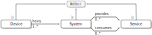
\includegraphics[scale=0.9]{figures/device-system-service}
  \caption{
    Hardware devices have, or \textit{host}, software systems, which \GlossaryHyperRef{provider-service}{provide} services.
    Each of these is an artifact.
  }
  \label{fig:device-system-service}
\end{figure}

  \vspace*{-3mm}

\subsection{Service Provision and Consumption}

Communication between systems is formulated in terms of the \GlossaryHyperRef{provider-service}{provision} and \GlossaryHyperRef{consumer-service}{consumption} of services, as depicted in Figure \ref{fig:service-consumption}.
When a system \textit{provides} a service, it makes it available to other systems through \GlossaryHyperRef{interface-service}{service interfaces}.
Other systems can \textit{consume} its services by sending \GlossaryHyperRef{message}{messages} to the interfaces of those services.
When a service interface receives a message, it \GlossaryHyperRef{routing-message}{routes} it to the specific function it targets.
That functions must ensure that the message conforms to its \GlossaryHyperRef{protocol-function}{protocol} and \GlossaryHyperRef{policy-function}{policies} before concretely handling it.
Function protocols establish what messages must contain and when they may be sent in relation to other messages, while policies establish what other conditions must be satisfied for the \GlossaryHyperRef{invocation-function}{function invocation} to be permitted.
In other words, a message satisfying a function protocol guarantees that the message is understood by its receiving function, while a message satisfying certain policies guarantees that the activity it would trigger is occurring under desirable conditions.
A policy may require that certain \GlossaryHyperRef{service-quality-of}{quality-of-service} guarantees can be met, or that the sender is properly authorized, among many other possible examples.

\begin{figure}[ht!]
  \centering
  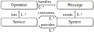
\includegraphics[scale=0.9]{figures/service-consumption}
  \caption{
    A system consumes a service by sending a message to its interface, which routes it to a function.
  }
  \label{fig:service-consumption}
\end{figure}

\subsection{System Composition}

When certain systems consume each other's services, those systems form a \GlossaryHyperRef{system-of-systems}{system-of-systems}, as illustrated in Figure \ref{fig:system-of-systems-small}.
That system-of-systems becomes able to perform activities none of its constituent \GlossaryHyperRef{subsystem}{subsystems} could perform on its own.
While there are many ways it could be relevant to structure systems in relation to each other, two are of particular significance in the context of the Arrowhead framework.
These are (1) the \GlossaryHyperRef{cloud-local}{local cloud}, and (2) the \GlossaryHyperRef{system-of-local-clouds}{system-of-local-clouds}.
A \textit{local cloud} is a pool of \GlossaryHyperRef{resource}{resources}, managed by systems, where at least one pooled resource is \GlossaryHyperRef{resource-local}{local}.
A \textit{local resource} derives its value from its physical \GlossaryHyperRef{property}{properties}.
Furthermore, all local clouds have at least one \GlossaryHyperRef{boundary-local}{\textit{local boundary}}, which is a physical property that distinguishes artifacts inside the cloud from those outside it.
A local cloud may also have \GlossaryHyperRef{resource-virtual}{virtual resources} and \GlossaryHyperRef{boundary-virtual}{virtual boundaries}.
Raw materials, drones, and other systems are a few examples of resources.
Boundaries may be formed by physical location, electronic certificate issuance, among many other possible examples.
A system-of-local-clouds emerges when distinct local clouds consume each other's services to perform new activities neither of the local clouds could perform on its own.

\begin{figure}[ht!]
  \centering
  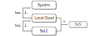
\includegraphics[scale=0.9]{figures/system-of-systems-small}
  \caption{
    The two primary kinds of systems-of-systems (SoS): the local cloud and the system-of-local-clouds (SoLC).
  }
  \label{fig:system-of-systems-small}
\end{figure}
